\section{Introduction}

The Reduced Area Medical Rectangular Oncological Device (RAMROD) shown in Figure \ref{fig:ram} is a proposed proton synchrotron for treatment of cancer patients.  
The device will deliver up to 2
Gray per second (\gs) to a 1 $mm^3$ tumor area.  The beam will originate in a 50 mA ion source, will be accelerated through a radio frequency quadropole (RFQ) and 
a drift tube linear accelerator (DTL) up to 7~\mev of energy. The beam will be injected into the synchrotron lattice, and accelerated to 250~\mev.  The sextopole 
magnet will be ramped to create the specific ``Third order resonance'' 
beam shape needed for a slow extraction over a few seconds. The extraction is 
performed by placing a thin electrostatic septum made of tungsten wire 
at a point where a single arm of the 3rd order resonance will intersect the field region.  These
particles will receive a ``kick'' equivalent to the voltage across the septum 
and begin moving away from the central beam.  Further down the extraction line there will be a thin magnetic septum to further bend the extracted
particles into the downstream beam pipe and toward the treatment area.  Using this method a constant dose can be delivered over several seconds to a target area.  
The depth of 
proton penetration can be adjusted by either placing a suitable moderating material before the patient, or reducing the energy of the extracted beam.  The beam may be 
scanned over a small area during the several second extraction in order to deliver dose in a grid to different parts of the tumor.  
\begin{figure}[h]
  \begin{center}
    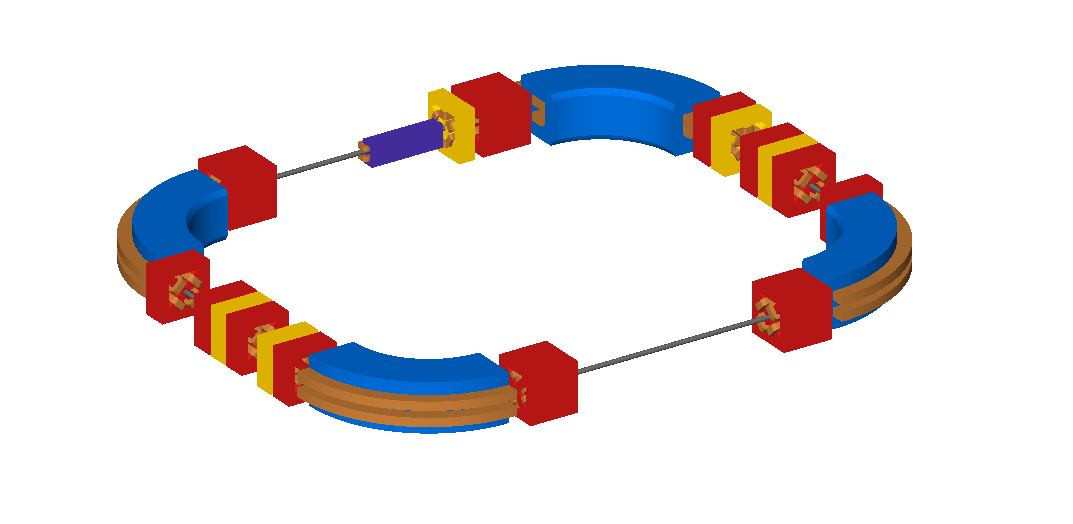
\includegraphics[width=0.9\textwidth]{ramrod.png}
    \caption{A computer drawing (created in BDSIM) of the proposed synchrotron.  The dipole magnets are shown in blue,
    the quadropoles are shown in red, and the sextopoles are shown in yellow.  The extraction septum is shown in purple. The RF system can be placed flexibly, however 
  it is expected to be located opposite the extraction septum, where the most free space exists.}
  \end{center}
  \label{fig:ram}
\end{figure}
Operation in scanning mode would require a higher beam intensity in order to deliver the required dose to each scan point.  Higher intensity is possible through the choice
of ion source, injection scheme and extraction time. 

The proton source is an Ion source similar to the one used at the SNS in ORNL.  The system is capable of producing 50mA of protons, 
which would provide $~3*10^{17}$ protons per second.  The 1 $mm^3$ of tumor area is approximately 1 mg of water, which would require $5*10^4$ protons per second to 
reach the nominal dose rate.  The slow extraction of the beam means that a fractional amount is extracted per turn, therefore we require a beam intensity of 
$>1*10^8$ for a 1000 turn extraction, pessimistically assuming 50\% extraction efficiency.  In order to keep the space charge tune shift smaller than 
$\nu_{sc} \le 0.2$ the machine is limited to approximately $1*10^{11}$ protons if operated in single bunch mode. This limitation 
only affects the length of time a single fill can be used for treatment. 
The major parameters of the accelerator are listed in Table \ref{tab:major}.  
\begin{table}[!hbt]
  \centering
  \begin{tabular}{lcrr}
    \hline 
    \textbf{Beam parameters}&\textbf{Unit}  &\textbf{Injection} &\textbf{Extraction}\\                        
    \hline \hline
    Kinetic energy      & MeV       & 7.0       & 250       \\
    $\beta_{rel}$     &       & 0.12 & 0.61   \\
    $\gamma_{rel}$      &       & 1.007         &1.267  \\
    Circumference   & m   &   22.8      & 22.8    \\
    Revolution period   & $\mu$s    & 0.63        &0.124    \\
    Magnetic rigidity   & T.m     & 0.38        &2.43 \\
    $\#$ bunches      &       &1        &1  \\
    Transverse normalized emittance (rms)\footnote{The emittance specifications might need to be increased based on the ion source and the space charge 
    effects for an intensity of $10^{11}$~p+. } & $\mu$m    & 2       &2\\
    Max. intensity  &   $10^{10}$~p+  &   1   & 1\\

    \hline
  \end{tabular}
  \caption{RAMROD beam parameters at injection and extraction.}
  \label{tab:major}
\end{table}



\section{Lattice}
The major design consideration was to keep the lattice size smaller than a large room, which suits a rectangular shape.  The 4 main steering dipoles making up the
corners, with about 23m around the whole ring.  Two straight sections are longer than the others (7m and 4m respectively), leaving free space for beam 
monitoring equipment and injection/extraction septa and magnets.  The longer straights are designed to be dispersion free regions to easily match injected beams
and the RF cavity with zero momentum spread.  Additionally the resonant sextopole for slow extraction will operate in a dispersion zero region.
The beam tunes should be far from any resonances, so that during the slow extraction, the tune can be adjusted in order to extract more of the beam.
The other sextopoles operate in a non-zero dispersion region in order to change the chromaticity of the beam.  One sextopole is installed where it can effect
$\beta_y$ strongly, and the other so that it may change primarily $\beta_x$.  The dipole magnets are designed to contain large non-superconducting copper loops
which produce $1.7 Tesla$ over a length of $2.2 m$. A small aperture in the $y$ direction strongly reduces the required current in the dipoles, and so a small 
$\beta_y$ is designed into the machine.  
\begin{figure}[h] 
  \begin{center}
    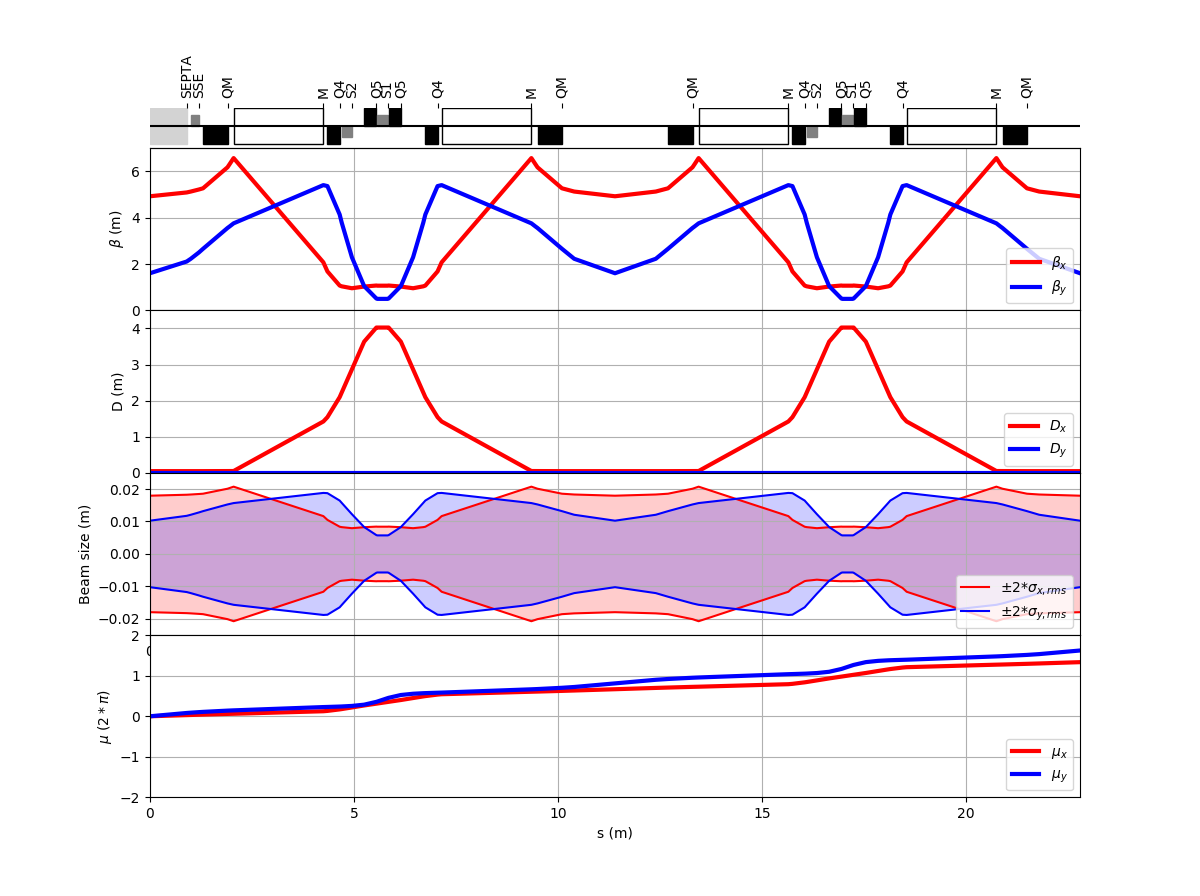
\includegraphics[width=0.45\textwidth]{twiss_33.png}
    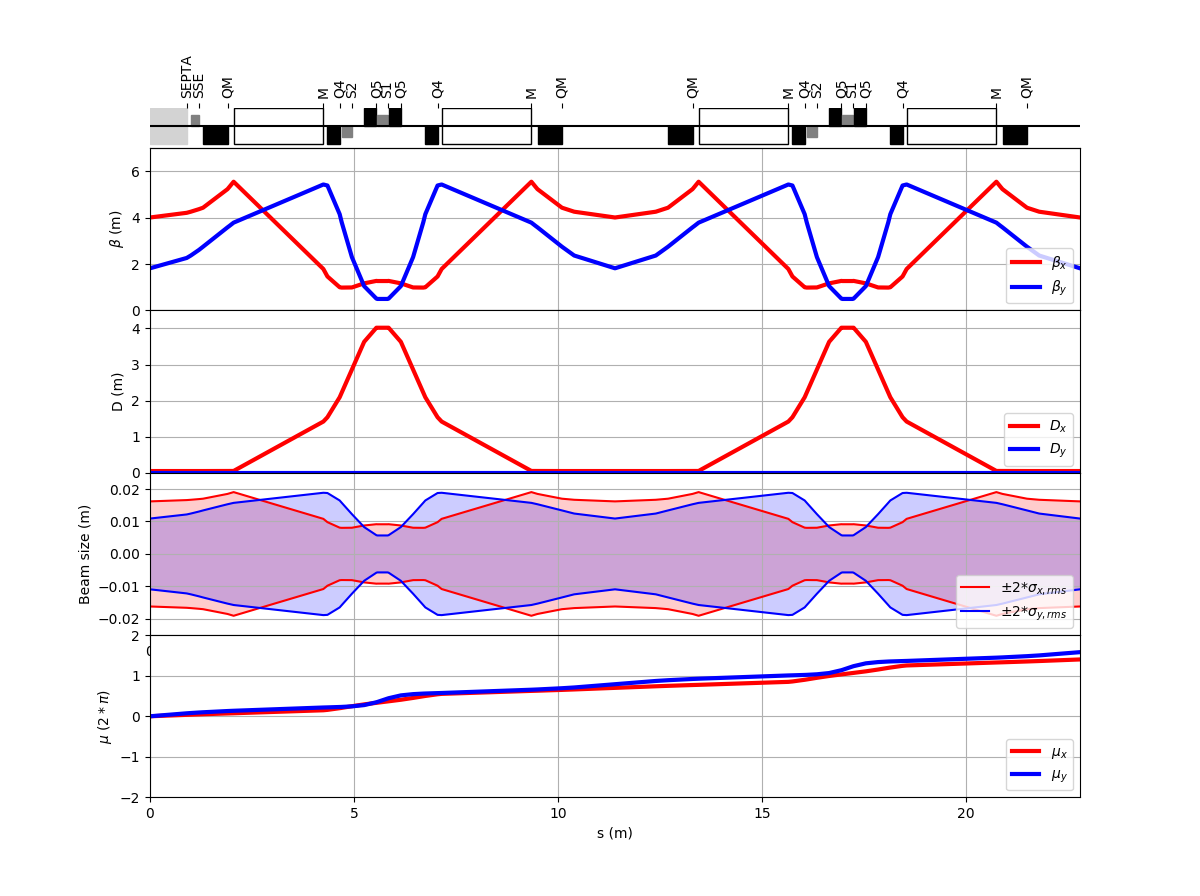
\includegraphics[width=0.45\textwidth]{twiss_40.png}
    \caption{The synchrotron lattice at two working points, $\nu_x = 1.33$ on the left and $\nu_x = 1.40$ on the right. 
      The left image shows the synchrotron after injection and during ramp.  The right
      image shows the synchrotron after the slow extraction.  The tune is adjusted during the extraction in order to move more central particles into
    the septum region. }

  \end{center}
  \label{fig:lat}
\end{figure}

\subsection{Design}
The synchrotron lattice can be seen in Figure \ref{fig:lat} along with the betatron tunes, dispersion and beam size.  The large white boxes correspond to the dipole
magnets, the dark boxes labeled Q correspond to quadropoles, and the boxes labeled S correspond to sextopoles.  The box labeled SEPTA is the beginning of the 
electromagnetic septum.  The design was completed in MAD-X, a lattice simulation software.  The 4 large dipoles provide weak focusing to the $\beta_x$ function which 
can be seen in its evolution in Figure \ref{fig:lat}.  The weak focusing goes with $1/\rho^2$ where $\rho = B * q/p = 1.4m$.  Edge angles of $\theta = 13^\circ$ provide
so called ``edge focusing'' in the $\beta_y$ function, which provides a majority of the focusing in that direction for this lattice. Two double bend acromat (DBA) cells
are included in the lattice to create straight  sections where dispersion is zero.  
\subsection{Apertures} 
Figure \ref{fig:lat} show the $2\sigma$ beam size at the injection and extraction points, magnet apertures must be made larger than this area.  The magnet alignment
uncertainty was not included in this study. The assumed rms-emittance is 2 mm-mrad, however this value is dependant on intensity of the beam, and might need to 
be re-evaluated if a long term high intensity operation is needed.  A larger emittance will require larger magnet apertures, which will need to be designed with
more wire loops or longer length in order to maintain their non-superconducting, and therefore cheaper and easier to maintain, nature.  
\subsection{RF}
The RF system is assumed to be locate in one of the longer straight sections of the lattice.  The RF Voltage should be chose to allow for sub 1-second ramp times which
is quite feasible with the listed revolution period in Table \ref{tab:major}.  A minimum of 250V can be supplied each revolution, however a higher voltage RF cavity 
would allow the ramp time to easily shrink by a factor of two or three. 
\subsection{Slow Extraction}
The resonant sextopole which will drive the slow extraction is placed in a region of zero dispersion to avoid resonance excursion by off momentum particles.  The 
electrostatic septum is also placed in a region of zero dispersion, such that the beam undergoes a phase advance of $\frac{5\pi}{2}$ so that only a single arm of
the third order resonant beam will be extracted each turn.  A length of 1m is reserved for the electrostatic septum and magnetic septum, however the total length
needed should be evaluated further.  There is room to expand the septum area upstream if there is not enough space to fit the extraction magnets next to the 
corner dipole.  
\subsection{Injection}
The injection devices are not included in the current study but are assumed to take up the long section across from the extraction area where there is room to add 
a kicker magnet.  A single turn injection is foreseen, since the ion source is capable of enough current to provide $~1e11$ protons in half of a turn which approaches
the space charge limits discussed earlier.  However a multi turn injection could be utilized if a weaker ion source is desired, with no major change in the lattice. The
multi-turn injection would require the usage of closed-orbit bumper magnets as well as an injection kicker.  The bumper magnets require a spacing of $\pi$ with respect
to each other, and therefor cold be placed in the middle of the Double Bend Acromats on either side of the injection area.   
 
\section{Conclusion and Outlook}
A small footprint medical synchrotron was presented and discussed.  Not all aspects are fully considered in this report, but note is made where further
design is needed.  The guiding principle was the reduced area, having a high current ion source allows for single-turn injection and a slow extraction over several
seconds.  The dispersion zero region adds flexibility for injection and extraction mechanics, however finding areas of appropriate phase advance outside the DBAs is 
difficult.  
 
\section{Appendix A: Magnet parameters and currents}

\begin{table}[]
  \caption{Hardware Parameters for the Main Dipoles at Injection and Extraction Energy.}
  \centering
  \begin{tabular}{@{}llll@{}}
          \toprule
          & \textbf{Unit} & \textbf{7 MeV} & \textbf{250 MeV} \\ 
          \hline \hline

          Length           & m    & 2.2   & 2.2     \\
          $B$              & T    & 1.735 & 1.735   \\
          $A_y$            & cm   & 2.2   & 2.2     \\
          $N \cdot I$      & kA   & 9.6   & 60.7    \\
          Coils            &      & 2     & 2       \\
          Turns            &      & 16    & 16      \\
          Current per wire & kA   & 0.299 & 1.9     \\ \bottomrule
        \end{tabular}
      \end{table}
      \label{tab:bend}

      \begin{center}
        \begin{table}[]
          \caption{Hardware Parameters for the Quadrupoles at Injection and Extraction Energy.}
          \begin{tabular}{@{}lllllllll@{}}
                  \toprule
                  &      & \multicolumn{3}{l}{QM (optics matching)} & \multicolumn{2}{l}{Q4} & \multicolumn{2}{l}{Q5} \\ \midrule
                  Energy      & MeV  & 7   & 250 (1.4) & 250 (1.33) & 7     & 250     & 7      & 250     \\
                  Length        & m    & 0.6     & 0.6           & 0.3            & 0.3       & 0.3        & 0.3       & 0.3        \\
                  $k$           & 1/m  & -0.185  & -0.185        & -0.253         & -2.55     & -2.555     & 2.195     & 2.195      \\
                  $g$           & T/m  & -0.07   & -0.5          & -0.61          & -0.97     & -6.2       & 0.84      & 5.33       \\
                  Aperture max  & cm   & 2.5     & 2.5           &  2.5              & 2.5       & 2.5        & 2.5       & 2.5        \\
                  $B_{poletip}$ & mT   & -0.002  & -0.011        & -0.015         & -0.024    & -0.155     & 0.021     & 0.133      \\
                  $N \cdot I$   & kA   & -0.0176 & -0.112        & -0.153         & -0.243    & -1.54      & 0.208     & 1.33       \\ \bottomrule
                \end{tabular}
                \label{tab:quad}
              \end{table}

            \end{center}

            \begin{center}
              \begin{table}[]
                \centering
                \caption{Hardware Parameters for the Chromatic Correction Sextupoles at $\nu_x=1.4$ and $\nu_x=1.33$.}
                \begin{tabular}{@{}llllll@{}}
                        \toprule
                        &         & \multicolumn{2}{l}{S1} & \multicolumn{2}{l}{S2} \\ \midrule
                        Energy        & MeV     & 250 (1.4) & 250 (1.33) & 250 (1.4) & 250 (1.33) \\
                        Length        & m       & 0.25      & 0.25       & 0.25      & 0.25       \\
                        $S$, normal.  & 1/m$^2$ & 13.6      & 18.3       & -14.0     & -15.7      \\
                        $S$           & T/m$^2$ & 70        & 100        & -72       & -80        \\
                        Aperture max  & cm      & 2.5       & 2.5        & 2.5       & 2.5        \\
                        $B_{poletip}$ & mT      & 0.02      & 0.03       & -0.02     & -0.02      \\
                        $N \cdot I$   & kA      & 0.136     & 0.194      & -0.141    & -0.158     \\ \bottomrule
                      \end{tabular}
                      \label{tab:sext}
                    \end{table} 
                  \end{center}{}
